% Discrete Curvature Approximation
\section{Discrete Curvature Approximation}
The concept of ``deviation'' as defined above is relatively 
straightforward and intuitive. However, another related way of describing 
``how well'' a \textit{discretization} represents a \textit{curve} is the 
degree to which the discrete representation approximates curvature -- 
where curvature is defined as the amount of ``bend'' in a \textit{curve} or surface, or ``how much'' a \textit{curve} or surface ``differs'' from a straight line or plane (words in quotes are subject to gradation). First, however, curvature must be defined in such a way that a discrete approximation is meaningful and appropriate. In relevant literature there are many ways to estimate curvature \cite{hermann07}. Some of it bears repeating because it is germane to what is being discussed here: Consider the following planar \textit{curve}, C, at point P. At a given point P there exists an osculating circle, O, of radius r such that the circle has the same tangent as the \textit{curve} C as well as the same radius of curvature \cite{gray97}. \\

\begin{figure}[h!]
  \center{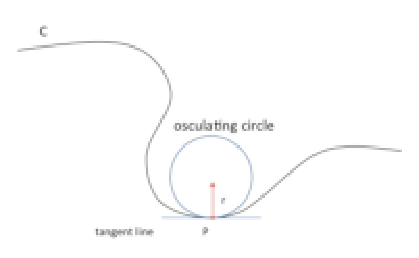
\includegraphics
    {Figures/OsculatingCircle.eps}}
  \caption{\label{OsculatingCircle} Osculating Circle of a Planar Curve}
\end{figure}

\noindent Just as the tangent line is the line best approximating a \textit{curve} at a point, the osculating circle is the best circle that approximates the \textit{curve} a point. Ignoring degenerate \textit{curve}s such as straight lines, the osculating circle of a given \textit{curve} at a given point is unique \cite{gray97}. The radius, r, of the osculating circle at a given point on a \textit{curve} is equal to the radius of curvature, R, which is the reciprocal of curvature, $\kappa$--sometimes called the ``first curvature'' \cite{kreyszig91}. For a two-dimensional \textit{curve} of the form $y=f(x)$, the equation for curvature is:
\[ 
R=\frac{1}{\kappa} \textnormal{, where } 
\kappa=\frac{\frac{d^2y}{dx^2}}{[1+\frac{dy}{dx}^2 ]^\frac{3}{2}}. 
\]
\noindent This quantity, $kappa$, necessarily includes the calculation of 
derivatives which, depending on the representation of the underlying geometrical description, could be relatively costly. Therefore, this is avoided by defining this radius of curvature on a segment or at a point in the \textit{discretization} without the use of derivatives. This is discussed in the following paragraphs.

A value of curvature can be calculated for each edge in the \textit{discretization} by considering the corresponding osculating circle on a given edge. The osculating circle here (circle, Figure 2) can be approximated by considering the circumscribed circle (circumcircle) \cite{casey1888} defined by the two end points of the edge, P0 and P1, and a point, P, between them in the \textit{curve} parameterization—the radius of the circumcircle will be referred to as the discrete radius of curvature.

\begin{figure}[h!]
  \center{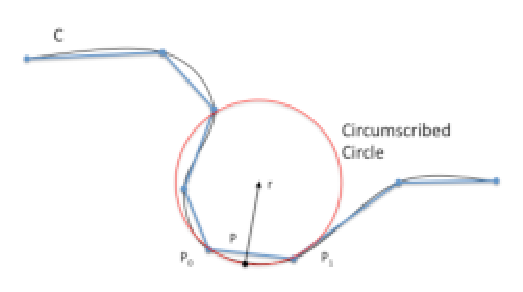
\includegraphics
    {Figures/CircumscribedCircle.eps}}
  \caption{\label{CircumscribedCircle} Caption}
\end{figure}

\noindent The method of choosing this point, P, and its importance to an accurate mesh refinement will be detailed later. This definition/approximation of the radius of curvature of the \textit{curve}/\textit{discretization} is useful for this application, but exhibits scale-dependence. The discrete radius of curvature alone is not sufficient to determine how well a segment approximates the curvature. The discrete radius of curvature must be given some context. In other words: it must be compared to the local feature size in order to determine if the segment is an accurate representation. Another problem with comparing the radius of curvature and the discrete radius of curvature is that as the \textit{discretization} becomes more refined the discrete radius of curvature approaches infinity and therefore diverges from the analytical value at that point. Stated another way, as the sum of the length of the segments in the \textit{discretization} converges to the actual length of the \textit{curve}, the discrete radius of curvature of each segment approaches infinity. Therefore, a quantity is needed that is scale-independent that converges to a computer-representable value as the \textit{discretization} becomes more refined.

Consider a circular segment, which represents the \textit{curve} 
$s$.  The corresponding chord, which represents a segment in the 
\textit{discretization}--$a$, and saggitta--which represents 
the ``deviation'' of the segment away from the \textit{curve} $h$
is shown in Figure~\ref{CircleGeometry}.

\begin{figure}
  \center{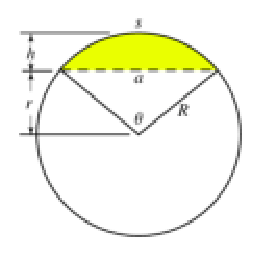
\includegraphics
    {Figures/CircleGeometry.eps}}
  \caption{\label{CircleGeometry} Caption}
\end{figure}.

\begin{theorem}
As the length of $a$ approaches the length of $s$, the length of $h$ goes 
to zero, therefore the radius of the circle, $R$, goes to infinity.  
\end{theorem}

\begin{proof}
First, 
\begin{eqnarray}
\begin{array}{lcl}
a & = & \sqrt{R^2+r^2}=2*\sqrt{(h*(2*R-h)}.
\end{array}
\end{eqnarray}
Upon rearranging, we obtain
\begin{eqnarray}
\begin{array}{lcl}
R & = & \frac{(\frac{a}{2})^2*\frac{1}{h}+h}{2}=
\frac{a^2+4*h^2}{8*h}=\frac{a^2}{8*h}+\frac{h}{2}.
\end{array}
\end{eqnarray}
Finally,
\begin{eqnarray}
\begin{array}{lcl}
\lim_{h\to0} (\frac{a^2}{(8*h)}+\frac{h}{2}) & = & \infty.
\end{array}
\end{eqnarray}
\end{proof}

Given the aforementioned proof, if the discrete curvature radius is 
divided by the length of the corresponding segment on the \textit{curve}, 
then it’s value approaches zero. This is a scale independent measure that 
converges to a computer representable number as the 
\textit{discretization} approaches the length of the \textit{curve}. The 
parameter is known as the curvature ratio. It is an intuitive measure that 
relates ``how far'' the \textit{curve} deviates from the segment that is representing it as the ratio of those lengths. Consider a point on a \textit{curve} between two endpoints of a segment of a \textit{discretization}, as seen in Figure-\ref{CurvatureRatio}. The length of the segment, $L_i$, is the distance from $P_0$ to $P_1$. The perpendicular distance between the point on the \textit{curve} between the end points and the segment is $L_c$. The three points define a curvature ratio through the ratio of $L_c$ to $L_i$.

\begin{figure}[h!]
  \center{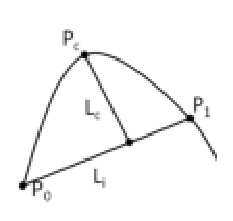
\includegraphics
    {Figures/CurvatureRatio.eps}}
  \caption{\label{CurvatureRatio} $curvature ratio=  \frac{L_c}{L_i}$ 
\cite{mclaurin10}}
\end{figure}

(pattern recognition is a field that has some research in this area)
